
% UC... specificare App o Server -> UCA / UCS

\centering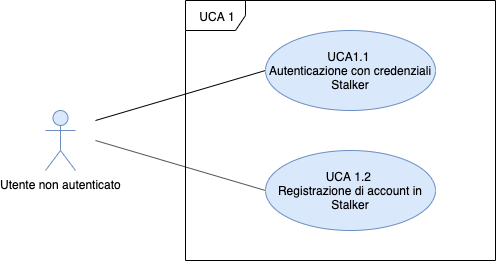
\includegraphics[scale=0.8]{sezioni/UseCase/Immagini/Panoramica.png}
\section{UCA  1}%kite level
\begin{itemize}
\item \textbf{Nome:} Accesso all'applicazione
\item \textbf{Attori primari:} Utente non autenticato
%\item \textbf{Attori secondari:}%opzionale
\item \textbf{Precondizione:} L’utente non è autenticato
\item \textbf{Postcondizione:} L’utente viene autenticato all’interno del sistema 
\item \textbf{Scenario principale:} L'utente non identificato può scegliere se registrarsi nel sistema oppure se possiede già un account può fare il login nell'applicazione %cosa potrebbe fare l'utente con il UC, descrizione
%\item \textbf{Estensioni:}
\item \textbf{Flusso di eventi:}
    \begin{enumerate}
        \item UCA 1.1;
        \item UCA 1.2;
    \end{enumerate}

\end{itemize}

\newpage
\centering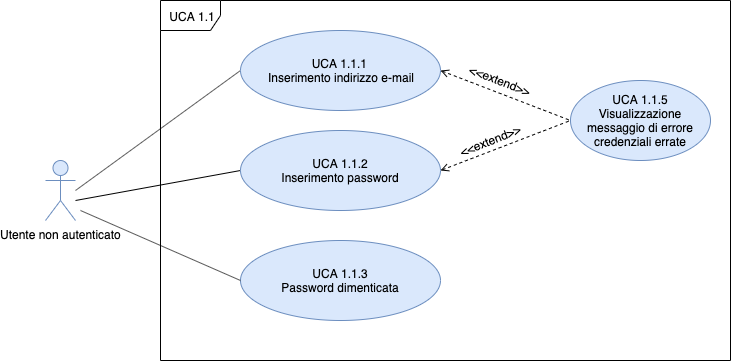
\includegraphics[scale=0.4]{sezioni/UseCase/Immagini/Login.png}
\subsection{UCA 1.1}%sea level
\begin{itemize}
\item \textbf{Nome:} Autenticazione con credenziali Stalker
\item \textbf{Attori primari:} Utente non autenticato
%\item \textbf{Attori secondari:}%opzionale
\item \textbf{Precondizione:} L’utente non è autenticato
\item \textbf{Postcondizione:} L’utente viene autenticato all’interno del sistema e può accedere all'applicazione
\item \textbf{Scenario principale:} L’utente non autenticato inserisce l’indirizzo e-mail e password per autenticarsi attraverso la dashboard iniziale%cosa potrebbe fare l'utente con il UC, descrizione
\item \textbf{Flusso di eventi:} %elenco puntato
  \begin{enumerate}
        \item UCA 1.1.1;
        \item UCA 1.1.2;
        \item UCA 1.1.3;
        \item UCA 1.1.4;
    \end{enumerate}
\item \textbf{Estensioni:}
	\begin{enumerate}
		\item UCA 1.1.5;
	\end{enumerate}
%\item \textbf{Inclusioni:}
\end{itemize}

\subsubsection{UCA 1.1.1}%fish level
\begin{itemize}
\item \textbf{Nome:} Inserimento indirizzo e-mail
\item \textbf{Attori primari:}  Utente non autenticato
%\item \textbf{Attori secondari:}%opzionale
\item \textbf{Precondizione:}  L’utente non è autenticato
\item \textbf{Postcondizione:}  L’utente ha inserito il proprio indirizzo e-mail
\end{itemize}

\subsubsection{UCA 1.1.2}%fish level
\begin{itemize}
\item \textbf{Nome:} Inserimento password
\item \textbf{Attori primari:} Utente non autenticato
%\item \textbf{Attori secondari:}%opzionale
\item \textbf{Precondizione:} L’utente non è autenticato
\item \textbf{Postcondizione:} L’utente ha inserito la propria password
\end{itemize}

\subsubsection{UCA 1.1.3}%fish level
\begin{itemize}
\item \textbf{Nome:} Pulsante accedi
\item \textbf{Attori primari:} Utente non autenticato
%\item \textbf{Attori secondari:}%opzionale
\item \textbf{Precondizione:} L'utente non autenticato
\item \textbf{Postcondizione:} L'utente ha fatto richiesta per essere autenticato dal sistema 
\end{itemize}

\subsubsection{UCA 1.1.4}%fish level
\begin{itemize}
\item \textbf{Nome:} Password dimenticata
\item \textbf{Attori primari:} Utente non autenticato
%\item \textbf{Attori secondari:}%opzionale
\item \textbf{Precondizione:}  L'utente non autenticato
\item \textbf{Postcondizione:} L'utente ha fatto richiesta per avviare la procedura di password dimenticata
\end{itemize}

\subsubsection{UCA 1.1.5}%fish level
\begin{itemize}
\item \textbf{Nome:} Visualizzazione messaggio di errore credenziali errate.
\item \textbf{Attori primari:} Utente non autenticato
%\item \textbf{Attori secondari:}%opzionale
\item \textbf{Precondizione:}  L'utente non autenticato
\item \textbf{Postcondizione:} L'utente visualizza un messaggio di errore a causa delle credenziali inserite in modo errato
\end{itemize}

\subsection{UCA 1.2}%sea level
\begin{itemize}
\item \textbf{Nome:} Registrazione di account in Stalker
\item \textbf{Attori primari:} Utente non autenticato
%\item \textbf{Attori secondari:}%opzionale
\item \textbf{Precondizione:} L’utente non é ancora registrato nel sistema.
\item \textbf{Postcondizione:} L’utente si è registrato e può accedere al sistema.
\item \textbf{Scenario principale:} L'utente non registrato compila il modulo di registrazione al fine di poter accedere al sistema;%cosa potrebbe fare l'utente con il UC, descrizione
\item \textbf{Flusso di eventi:} %elenco puntato
  \begin{enumerate}
        \item UCA 1.2.1;
        \item UCA 1.2.2;
        \item UCA 1.2.3;
        \item UCA 1.2.4;
    \end{enumerate}
\item \textbf{Estensioni:}
	\begin{enumerate}
		\item UCA 1.2.5;
		\item UCA 1.2.6 ;
		\item UCA 1.2.7; 
		\item UCA 1.2.8; 
	\end{enumerate}
%\item \textbf{Inclusioni:}
\end{itemize}
\centering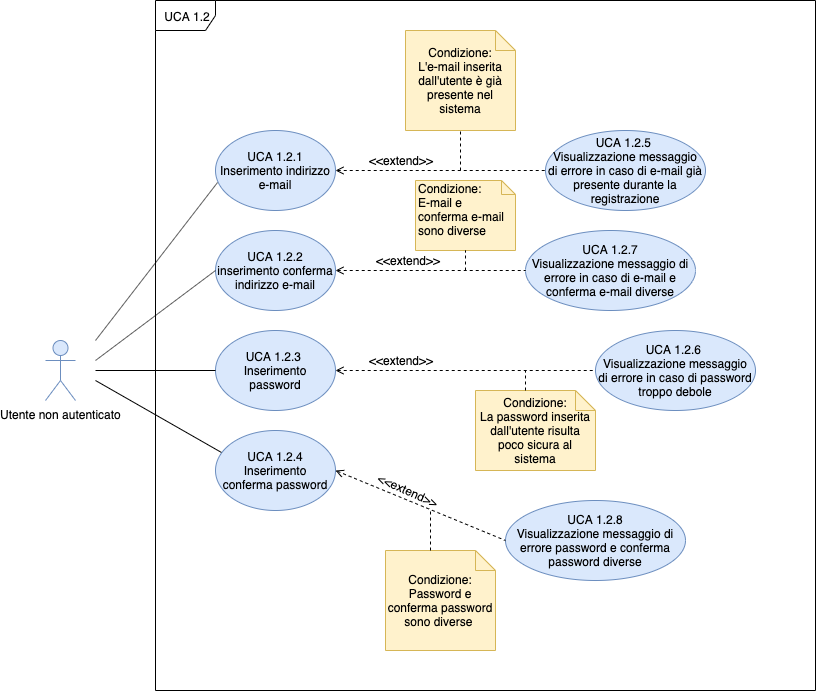
\includegraphics[scale=0.5]{sezioni/UseCase/Immagini/Registrazione.png}
\subsubsection{UC 1.2.1}%fish level
\begin{itemize}
\item \textbf{Nome:} Inserimento indirizzo e-mail
\item \textbf{Attori primari:} Utente non autenticato
%\item \textbf{Attori secondari:}%opzionale
\item \textbf{Precondizione:} L’utente non è registrato e il suo indirizzo e-mail non è ancora presente nel sistema
\item \textbf{Postcondizione:}  L’utente ha inserito il proprio indirizzo e-mail
\item \textbf{Estensioni:}
	\begin{enumerate}
		\item UCA 1.2.5
	\end{enumerate}
\end{itemize}

\subsubsection{UCA 1.2.2}%fish level
\begin{itemize}
\item \textbf{Nome:} Inserimento conferma indirizzo e-mail
\item \textbf{Attori primari:} Utente non autenticato
%\item \textbf{Attori secondari:}%opzionale
\item \textbf{Precondizione:} L’utente non è registrato e la sua conferma indirizzoe-mail non è ancora presente nel sistema
\item \textbf{Postcondizione:}  L’utente ha inserito la conferma dell'indirizzo e-mail
\item \textbf{Estensioni:}
	\begin{enumerate}
		\item UCA 1.2.7;
	\end{enumerate} 
\end{itemize}


\subsubsection{UCA 1.2.3}%fish level
\begin{itemize}
\item \textbf{Nome:} Inserimento password
\item \textbf{Attori primari:} Utente non autenticato
%\item \textbf{Attori secondari:}%opzionale
\item \textbf{Precondizione:} L’utente non è registrato e la sua password non è ancora presente nel sistema
\item \textbf{Postcondizione:} L’utente ha inserito una password
\item \textbf{Estensioni:}
	\begin{enumerate}
		\item UCA 1.2.6;
	\end{enumerate}
\end{itemize}

\subsubsection{UCA 1.2.4}%fish level
\begin{itemize}
\item \textbf{Nome:} Inserimento conferma password
\item \textbf{Attori primari:} Utente non autenticato
%\item \textbf{Attori secondari:}%opzionale
\item \textbf{Precondizione:} L’utente non è registrato  e la conferma password non è ancora definita
\item \textbf{Postcondizione:} L’utente ha inserito la conferma della password
\item \textbf{Estensioni:}
	\begin{enumerate}
		\item UCA 1.2.8;
	\end{enumerate}
\end{itemize}

\subsubsection{UCA 1.2.5}%fish level
\begin{itemize}
\item \textbf{Nome:} Visualizzazione messaggio di errore in caso di e-mail già presente durante la registrazione
\item \textbf{Attori primari:} Utente non autenticato
%\item \textbf{Attori secondari:}%opzionale
\item \textbf{Precondizione:} L’utente non è registrato ed ha inserito nel campo indirizzo e-mail un valore già presente nel sistema
\item \textbf{Postcondizione:} L'indirizzo e-mail inserito dall'utente è già presente nel sistema, pertanto riceve un messaggio di errore 
\end{itemize}

\subsubsection{UCA 1.2.6}%fish level
\begin{itemize}
\item \textbf{Nome:} Visualizzazione messaggio di errore in caso di password troppo debole 
\item \textbf{Attori primari:} Utente non autenticato
%\item \textbf{Attori secondari:}%opzionale
\item \textbf{Precondizione:} L’utente non è registrato ed ha inserito una password poco sicura
\item \textbf{Postcondizione:} La password inserita dall’utente risulta essere poco sicura per il sistema, pertanto riceve un messaggio di errore.
\end{itemize}

\subsubsection{UCA 1.2.7}%fish level
\begin{itemize}
\item \textbf{Nome:} Visualizzazione messaggio di errore in caso di e-mail e conferma e-mail diverse
\item \textbf{Attori primari:} Utente non autenticato
%\item \textbf{Attori secondari:}%opzionale
\item \textbf{Precondizione:} L’utente non è registrato ed ha inserito nei campi relativi alla e-mail e conferma e-mail indirizzi di posta elettronica differenti 
\item \textbf{Postcondizione:} La e-mail inserita dall'utente è diversa da quella inserita nel campo conferma e-mail, pertanto riceve un messaggio di errore.
\end{itemize}

\subsubsection{UCA 1.2.8}%fish level
\begin{itemize}
\item \textbf{Nome:}  Visualizzazione messaggio di errore in caso di password e conferma password diverse
\item \textbf{Attori primari:} Utente non autenticato
%\item \textbf{Attori secondari:}%opzionale
\item \textbf{Precondizione:} L’utente generico non è registrato ed ha inserito nei campi relativi alla password e conferma password valori differenti
\item \textbf{Postcondizione:} La password inserita dall’utente è diversa da quella inserita nel campo conferma password, pertanto riceve un messaggio di errore.
\end{itemize}

